% Author: Vladimir Dusek
% Date: 18/12/2018

%%%%%%%%%%%%%%%%%%%%%%%%%%%%%%%%%%%%%%%%%%%%%%%%%%%%%%%%%%%%%%%%%%%%%

\documentclass[11pt, a4paper, titlepage]{article}
\usepackage[left=2cm, text={17cm, 24cm}, top=3cm]{geometry}
\usepackage[utf8]{inputenc}
\usepackage[czech]{babel}
\usepackage{pdfpages}
\usepackage[obeyspaces]{url}
\usepackage{framed}
\usepackage{float}
\usepackage{subcaption}

\setlength\parindent{0pt}

%%%%%%%%%%%%%%%%%%%%%%%%%%%%%%%%%%%%%%%%%%%%%%%%%%%%%%%%%%%%%%%%%%%%%

\begin{document}

\begin{titlepage}
    \begin{center}
    \begin{figure}[htb]
    \centering
    
\includegraphics[width=0.85\hsize]{images/fitlogo.pdf}
    \end{figure}
    \vspace{\stretch{0.382}}
    {\Huge Mikroprocesorové a vestavěné systémy} \\
    \bigskip
    {\LARGE Dokumentace k~projektu pro ARM-FITkit3} \\
    \bigskip
    {\Large Varianta: Aplikace modulu Random Number Generator Accelerator (RNGA)}
    \vspace{\stretch{0.618}}
    \end{center}
    {\Large \today \hfill Vladimír Dušek, xdusek27}
\end{titlepage}

%%%%%%%%%%%%%%%%%%%%%%%%%%%%%%%%%%%%%%%%%%%%%%%%%%%%%%%%%%%%%%%%%%%%%

\tableofcontents
\newpage

%%%%%%%%%%%%%%%%%%%%%%%%%%%%%%%%%%%%%%%%%%%%%%%%%%%%%%%%%%%%%%%%%%%%%

\section{Úvod}

Cílem projektu bylo vytvořit funkční aplikaci na platformě FitKit3 (Minerva) pro generování náhodných čísel pomocí modulu Random Number Generator Accelerator (RNGA). Vygenerovaná posloupnost čísel byla dála analyzována nástrojem Dieharder. \\

Pro potřeby projektu bylo nutné si prostudovat principy tvorby vestavěných aplikací pro mikrokontrolér Kinetis K60 s~jádren ARM Cortex-M4 fy Freescale. Implementace byla realizována ve vývojovém prostředí Kinetis Design Studio od společnosti NXP prostřednictvím programovacího jazyka C.

%%%%%%%%%%%%%%%%%%%%%%%%%%%%%%%%%%%%%%%%%%%%%%%%%%%%%%%%%%%%%%%%%%%%%

\section{Realizace}

V~této kapitole je popsána kompletní realizace projektu. Vývojové prostředí,  inicializace mikrokontroléru, popis modulu RNGA, programová logika aplikace a konfigurace nástroje Putty.


\subsection{Vývojové prostředí}

Projekt byl vyvíjen na operačním systému Microsoft Windows 10 ve vývojovém prostředí Kinetis Design Studio. Projekt byl vytvořen jako Processor Expert Project. \cite{NXP-IDE}


\subsection{Inicializace mikrokontroléru}

Inicializace mikrokontroléru proběhla podobně jako na cvičení, bylo provedeno základní nastavení hodin. Byly povoleny hodiny pro moduly UART5, RNGA a PORT-E, ten byl použit jako Transmitter pro UART5. Komunikace s~platformou byla navázáno pomocí aplikace Putty ve Windows a modulu UART5 na FITkitu3. UART5 byl inicializován podobně jako UART0 na cvičeních. Tedy baudrate 115\,200, 8 datových bitů a parita zakázána. \cite{IMP}


\subsection{Modul RNGA}

Modul RNGA (Random Number Generator Accelerator) slouží, jak už z~jeho názvu plyne, pro generování náhodných čísel. Má 4 registry, Control Register, Status Register, Entropy Register a Output Register. \cite{NXP-K60}


\subsubsection{Control Register}

Control Register je vstupní registr, kterým celý modul nastavujeme. Obsahuje 5 příznaků. První z~ních je Sleep, pokud je povolený, tak modul RNGA nic nezapisuje do výstupního Output Register, ten tedy budeme chtít vypnout. Další je Clear Interrupt, jeho povolením vyčistíme error interrupt a error status bit ve Status registru, opět budeme chtít nechat vypnutý. Příznak Interrupt Mask zamaskuje error interrupt, ten také nechceme povolit. Další je High Assurance, jeho povolením zamaskujeme oznámení o~porušení bezpečnosti, také nechceme. Poslední příznak GO povolíme a tím se do výstupního registru RNGA Output začnou zapisovat data.

\subsubsection{Status Register}

Status Register je read-only registr a reflektuje interní chování modulu RNGA. Obsahuje mnoho příznaků. My před přečtením hodnoty z~Output registru zkontrolujeme příznak Sleep, tedy že modul není ve sleep módu a příznak Output Register Level, tudíž že náhodné slovo (word) bylo zapsáno do Output registru.


\subsubsection{Entropy Register}

Entropy Register je pro změnu write-only registr a slouží pro vložení seedu pro generování. Explicitní seed od uživatele není povinný, ale doporučený. Jelikož chceme co nejvíce možné náhodné hodnoty seed zvolíme, využijeme standardní C funkci \path{time()}. \cite{TIME}


\subsubsection{Output Register}

Output Register je výstupní registr, který je dočasným uložištěm pro náhodně vygenerovaná data. Náhodné slovo je uložene do registru každých 256 taktů, není-li registr plný.


\subsection{Programová logika}

Po inicializaci potřebných modulů, která byla popsána výše, skončí náš program v~nekonečné smyčce, případně s~podmínkou pro konkrétní počet náhodných hodnot. V~každé iteraci jsou volány funkce, které zapíší do Entropy registru seed, zkontrolují potřebné příznaky ve stavovém registru, přečtou hodnotu z~Output registru a pošlou ji přes rozhraní UART5 na vzdálený terminál v~Putty. Hlavní smička je zachycena na obrázku~\ref{fig:source_code}.

\begin{figure}[H]
    \centering
    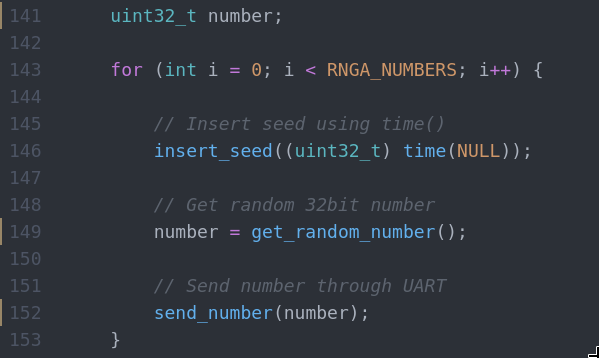
\includegraphics[width=.65\textwidth]{images/source_code.png}
    \captionof{figure}{Hlavní smička}
    \label{fig:source_code}
\end{figure}


\subsection{Konfigurace Putty}

Putty nastavíme odpovídajícím hodnotám z~inicializace mikrokontroléru. Pro pozdější analýzu můžeme v~Putty nastavit logování výstupu do souboru, který budeme později analyzovat. Více na obrázcích~\ref{fig:putty_1},~\ref{fig:putty_2},~\ref{fig:putty_3}.

\begin{figure}[H]
    \centering
    \begin{minipage}{.5\textwidth}
    \centering
    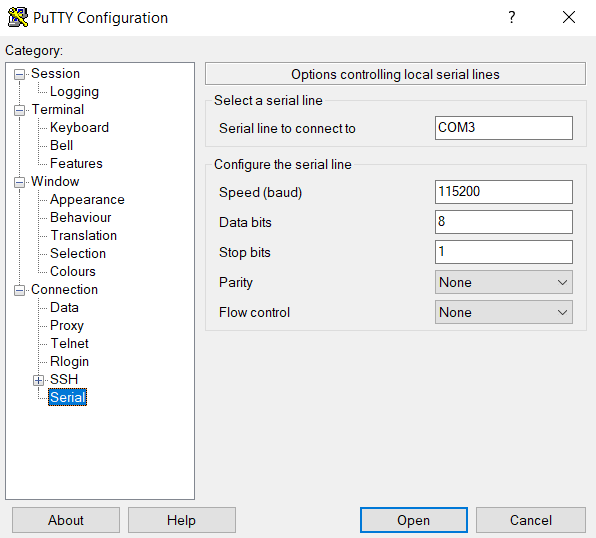
\includegraphics[width=.97\textwidth]{images/putty_1.png}
    \captionof{figure}{Serial connection type}
    \label{fig:putty_1}
    \end{minipage}%
    \begin{minipage}{.5\textwidth}
    \centering
    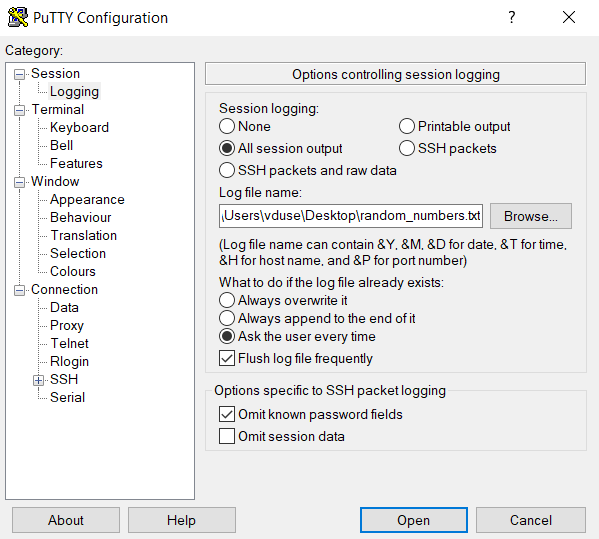
\includegraphics[width=.97\textwidth]{images/putty_2.png}
    \captionof{figure}{Logging}
    \label{fig:putty_2}
    \end{minipage}
\end{figure}

\begin{figure}[H]
    \centering
    \begin{minipage}{.5\textwidth}
    \centering
    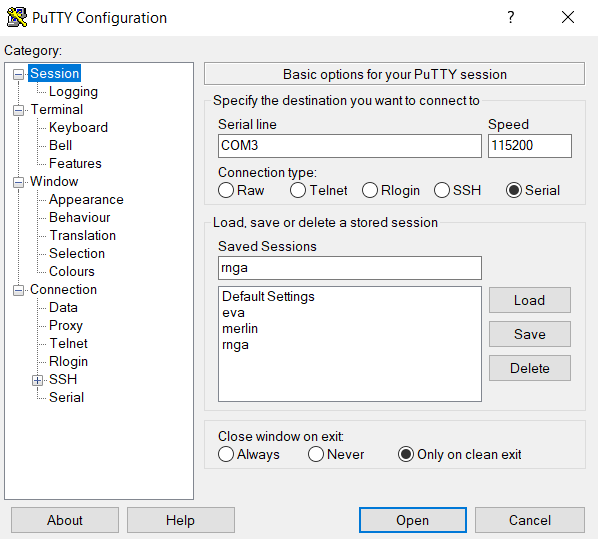
\includegraphics[width=.97\textwidth]{images/putty_3.png}
    \captionof{figure}{Session}
    \label{fig:putty_3}
    \end{minipage}
\end{figure}

%%%%%%%%%%%%%%%%%%%%%%%%%%%%%%%%%%%%%%%%%%%%%%%%%%%%%%%%%%%%%%%%%%%%%

\section{Analýza}

V~kapitole je popsána analýza vygenerovaných hodnot pomocí nástroje Dieharder.

\subsection{Vygenerovaná data}
Celkem bylo vygenerováno 11\,607\,870 náhodných 32 bitových hodnot. Generování trvalo zhruba 6 hodin času. Výsledkem je 136.3\,MB velký textový soubor.

\subsection{Dieharder}
Hodnoty byly analyzovány nástrojem Dieharder. Jedná se o~program pro výkonnostní testy generátorů náhodných čísel. Dieharder byl spuštěn s~přepínačem \path{-a}, kterým specifikujeme, že chceme všechny testy s~výchozím nastavením a přepínačem \path{-f}, kterým zadáváme soubor se vstupníma hodnotama. \cite{DIEHARDER}

\begin{framed}
    \path{$ dieharder -a -f random_numbers_32bit.txt}
\end{framed}

\subsection{Výsledky analýzy}
Kompletní výsledky analýzy si můžeme prohlédnout na obrázcích~\ref{tab:analysis_32b_1} a~\ref{tab:analysis_32b_2}. Celkem proběhlo 114 testů, z~toho 111 bylo označeno jako PASSED, 3 jako WEAK a žádný test neskončil jako FAILED. Dieharder funguje na principu statistickém testování hypotéz pomocí tzv. P-values (více vysvětleno např. v~\cite{DIEHARDER} a \cite{P-VALUE}). Naše hypotéza by měla říkat, že všechna čísla jsou generována se stejnou pravděpodobností. Náš generátor ovšem může generovat až $2^{32}$ různých hodnot, to je více než 4 miliardy. My vygenerovali pouze něco přes 11 miliónů, to pochopitelně pro 100\% spolehlivou analýzu nemůže být dostatečné množství.

%%%%%%%%%%%%%%%%%%%%%%%%%%%%%%%%%%%%%%%%%%%%%%%%%%%%%%%%%%%%%%%%%%%%%

\newpage

\begin{figure}[H]
    \fontsize{8pt}{10pt}\selectfont
    \begin{verbatim}
    #=============================================================================#
    #            dieharder version 3.31.1 Copyright 2003 Robert G. Brown          #
    #=============================================================================#
       rng_name    |           filename             |rands/second|
        mt19937    |    random_numbers_32bit.txt    |  8.20e+07  |
    #=============================================================================#
    test_name   |ntup| tsamples |psamples|  p-value |Assessment
    #=============================================================================#
       diehard_birthdays|   0|       100|     100|0.90069760|  PASSED
          diehard_operm5|   0|   1000000|     100|0.03577087|  PASSED
      diehard_rank_32x32|   0|     40000|     100|0.26050439|  PASSED
        diehard_rank_6x8|   0|    100000|     100|0.01374393|  PASSED
       diehard_bitstream|   0|   2097152|     100|0.35228093|  PASSED
            diehard_opso|   0|   2097152|     100|0.53339210|  PASSED
            diehard_oqso|   0|   2097152|     100|0.95438391|  PASSED
             diehard_dna|   0|   2097152|     100|0.29372942|  PASSED
    diehard_count_1s_str|   0|    256000|     100|0.99330963|  PASSED
    diehard_count_1s_byt|   0|    256000|     100|0.78685765|  PASSED
     diehard_parking_lot|   0|     12000|     100|0.29327315|  PASSED
        diehard_2dsphere|   2|      8000|     100|0.55743819|  PASSED
        diehard_3dsphere|   3|      4000|     100|0.99214949|  PASSED
         diehard_squeeze|   0|    100000|     100|0.37731548|  PASSED
            diehard_sums|   0|       100|     100|0.02791320|  PASSED
            diehard_runs|   0|    100000|     100|0.99395316|  PASSED
            diehard_runs|   0|    100000|     100|0.96359937|  PASSED
           diehard_craps|   0|    200000|     100|0.98789263|  PASSED
           diehard_craps|   0|    200000|     100|0.28685545|  PASSED
     marsaglia_tsang_gcd|   0|  10000000|     100|0.50453986|  PASSED
     marsaglia_tsang_gcd|   0|  10000000|     100|0.92598460|  PASSED
             sts_monobit|   1|    100000|     100|0.72316249|  PASSED
                sts_runs|   2|    100000|     100|0.50019629|  PASSED
              sts_serial|   1|    100000|     100|0.03055507|  PASSED
              sts_serial|   2|    100000|     100|0.96966912|  PASSED
              sts_serial|   3|    100000|     100|0.61484763|  PASSED
              sts_serial|   3|    100000|     100|0.10431401|  PASSED
              sts_serial|   4|    100000|     100|0.80511215|  PASSED
              sts_serial|   4|    100000|     100|0.95088735|  PASSED
              sts_serial|   5|    100000|     100|0.61501885|  PASSED
              sts_serial|   5|    100000|     100|0.98768492|  PASSED
              sts_serial|   6|    100000|     100|0.84929018|  PASSED
              sts_serial|   6|    100000|     100|0.98545960|  PASSED
              sts_serial|   7|    100000|     100|0.80194494|  PASSED
              sts_serial|   7|    100000|     100|0.57684535|  PASSED
              sts_serial|   8|    100000|     100|0.98411808|  PASSED
              sts_serial|   8|    100000|     100|0.59164623|  PASSED
              sts_serial|   9|    100000|     100|0.28148872|  PASSED
              sts_serial|   9|    100000|     100|0.58355523|  PASSED
              sts_serial|  10|    100000|     100|0.58433573|  PASSED
              sts_serial|  10|    100000|     100|0.56850611|  PASSED
              sts_serial|  11|    100000|     100|0.99970927|   WEAK
              sts_serial|  11|    100000|     100|0.70996297|  PASSED
              sts_serial|  12|    100000|     100|0.38858153|  PASSED
              sts_serial|  12|    100000|     100|0.54862380|  PASSED
              sts_serial|  13|    100000|     100|0.09580810|  PASSED
              sts_serial|  13|    100000|     100|0.67035516|  PASSED
              sts_serial|  14|    100000|     100|0.91588632|  PASSED
              sts_serial|  14|    100000|     100|0.48438498|  PASSED
              sts_serial|  15|    100000|     100|0.85726595|  PASSED
              sts_serial|  15|    100000|     100|0.92727368|  PASSED
              sts_serial|  16|    100000|     100|0.22358053|  PASSED
              sts_serial|  16|    100000|     100|0.71330339|  PASSED
    \end{verbatim}
    \caption{Analýza 32\,bit hodnot (část 1)}
    \label{tab:analysis_32b_1}
\end{figure}

%%%%%%%%%%%%%%%%%%%%%%%%%%%%%%%%%%%%%%%%%%%%%%%%%%%%%%%%%%%%%%%%%%%%%

\newpage

\begin{figure}[H]
    \fontsize{8pt}{10pt}\selectfont
    \centering
    \begin{verbatim}
             rgb_bitdist|   1|    100000|     100|0.61523046|  PASSED
             rgb_bitdist|   2|    100000|     100|0.33052474|  PASSED
             rgb_bitdist|   3|    100000|     100|0.32984712|  PASSED
             rgb_bitdist|   4|    100000|     100|0.96013281|  PASSED
             rgb_bitdist|   5|    100000|     100|0.80444629|  PASSED
             rgb_bitdist|   6|    100000|     100|0.31828218|  PASSED
             rgb_bitdist|   7|    100000|     100|0.26696280|  PASSED
             rgb_bitdist|   8|    100000|     100|0.39557538|  PASSED
             rgb_bitdist|   9|    100000|     100|0.61411068|  PASSED
             rgb_bitdist|  10|    100000|     100|0.98513528|  PASSED
             rgb_bitdist|  11|    100000|     100|0.51967868|  PASSED
             rgb_bitdist|  12|    100000|     100|0.28283173|  PASSED
    rgb_minimum_distance|   2|     10000|    1000|0.06329670|  PASSED
    rgb_minimum_distance|   3|     10000|    1000|0.77371244|  PASSED
    rgb_minimum_distance|   4|     10000|    1000|0.17139134|  PASSED
    rgb_minimum_distance|   5|     10000|    1000|0.56766873|  PASSED
        rgb_permutations|   2|    100000|     100|0.12041546|  PASSED
        rgb_permutations|   3|    100000|     100|0.33979486|  PASSED
        rgb_permutations|   4|    100000|     100|0.97860630|  PASSED
        rgb_permutations|   5|    100000|     100|0.99779028|   WEAK
          rgb_lagged_sum|   0|   1000000|     100|0.75083703|  PASSED
          rgb_lagged_sum|   1|   1000000|     100|0.38601635|  PASSED
          rgb_lagged_sum|   2|   1000000|     100|0.06783956|  PASSED
          rgb_lagged_sum|   3|   1000000|     100|0.84540760|  PASSED
          rgb_lagged_sum|   4|   1000000|     100|0.78262562|  PASSED
          rgb_lagged_sum|   5|   1000000|     100|0.76071502|  PASSED
          rgb_lagged_sum|   6|   1000000|     100|0.52301885|  PASSED
          rgb_lagged_sum|   7|   1000000|     100|0.48414317|  PASSED
          rgb_lagged_sum|   8|   1000000|     100|0.59987476|  PASSED
          rgb_lagged_sum|   9|   1000000|     100|0.47348194|  PASSED
          rgb_lagged_sum|  10|   1000000|     100|0.53757164|  PASSED
          rgb_lagged_sum|  11|   1000000|     100|0.99504480|   WEAK
          rgb_lagged_sum|  12|   1000000|     100|0.53423149|  PASSED
          rgb_lagged_sum|  13|   1000000|     100|0.02558795|  PASSED
          rgb_lagged_sum|  14|   1000000|     100|0.96109282|  PASSED
          rgb_lagged_sum|  15|   1000000|     100|0.30516226|  PASSED
          rgb_lagged_sum|  16|   1000000|     100|0.43580816|  PASSED
          rgb_lagged_sum|  17|   1000000|     100|0.63414810|  PASSED
          rgb_lagged_sum|  18|   1000000|     100|0.04200033|  PASSED
          rgb_lagged_sum|  19|   1000000|     100|0.79682877|  PASSED
          rgb_lagged_sum|  20|   1000000|     100|0.38978238|  PASSED
          rgb_lagged_sum|  21|   1000000|     100|0.32072971|  PASSED
          rgb_lagged_sum|  22|   1000000|     100|0.68588555|  PASSED
          rgb_lagged_sum|  23|   1000000|     100|0.90581383|  PASSED
          rgb_lagged_sum|  24|   1000000|     100|0.57830353|  PASSED
          rgb_lagged_sum|  25|   1000000|     100|0.67401272|  PASSED
          rgb_lagged_sum|  26|   1000000|     100|0.52167416|  PASSED
          rgb_lagged_sum|  27|   1000000|     100|0.01669872|  PASSED
          rgb_lagged_sum|  28|   1000000|     100|0.14404494|  PASSED
          rgb_lagged_sum|  29|   1000000|     100|0.31591798|  PASSED
          rgb_lagged_sum|  30|   1000000|     100|0.20703136|  PASSED
          rgb_lagged_sum|  31|   1000000|     100|0.10997257|  PASSED
          rgb_lagged_sum|  32|   1000000|     100|0.82936788|  PASSED
         rgb_kstest_test|   0|     10000|    1000|0.60597833|  PASSED
         dab_bytedistrib|   0|  51200000|       1|0.41758550|  PASSED
                 dab_dct| 256|     50000|       1|0.03974753|  PASSED
    Preparing to run test 207.  ntuple = 0
            dab_filltree|  32|  15000000|       1|0.45541597|  PASSED
            dab_filltree|  32|  15000000|       1|0.46641811|  PASSED
    Preparing to run test 208.  ntuple = 0
           dab_filltree2|   0|   5000000|       1|0.30251521|  PASSED
           dab_filltree2|   1|   5000000|       1|0.09723908|  PASSED
    Preparing to run test 209.  ntuple = 0
            dab_monobit2|  12|  65000000|       1|0.78664477|  PASSED
    \end{verbatim}
    \caption{Analýza 32\,bit hodnot (část 2)}
    \label{tab:analysis_32b_2}
\end{figure}

%%%%%%%%%%%%%%%%%%%%%%%%%%%%%%%%%%%%%%%%%%%%%%%%%%%%%%%%%%%%%%%%%%%%%

\newpage

\section{Analýza 8 bitových hodnot}

Pro věrohodnější testování jsme upravili náš program, aby generoval pouze 8\,bitové hodnoty.


\subsection{Vygenerovaná data}

Bylo vygenerováno 931\,847 čísel, velikost výsledného textového souboru byla pouze 4.3\,MB.


\subsection{Dieharder}
Hodnoty jsou analyzovány stejným způsobem.

\begin{framed}
    \path{$ dieharder -a -f random_numbers_8bit.txt}
\end{framed}

\subsection{Výsledky analýzy}
Kompletní výsledky analýzy si můžeme prohlédnout na obrázcích~\ref{tab:analysis_8b_1} a~\ref{tab:analysis_8b_2}. Tentokrát všech 114 testů skončilo úspěšně. 8 bitová čísla mohou nabývat pouze 256 možných hodnot, my vygenerovali téměř milion čísel. Tento počet byl naprosto dostatečný pro otestování výkonu generátoru náhodnosti. Z~výsledků je patrné, že náš program opravdu generuje náhodné hodnoty.

%%%%%%%%%%%%%%%%%%%%%%%%%%%%%%%%%%%%%%%%%%%%%%%%%%%%%%%%%%%%%%%%%%%%%

\newpage

\begin{figure}[H]
    \fontsize{8pt}{10pt}\selectfont
    \begin{verbatim}
    #=============================================================================#
    #            dieharder version 3.31.1 Copyright 2003 Robert G. Brown          #
    #=============================================================================#
       rng_name    |           filename             |rands/second|
        mt19937    |    random_numbers_8bit.txt     |  6.45e+07  |
    #=============================================================================#
    test_name   |ntup| tsamples |psamples|  p-value |Assessment
    #=============================================================================#
       diehard_birthdays|   0|       100|     100|0.23068546|  PASSED
          diehard_operm5|   0|   1000000|     100|0.96701400|  PASSED
      diehard_rank_32x32|   0|     40000|     100|0.27928836|  PASSED
        diehard_rank_6x8|   0|    100000|     100|0.53092485|  PASSED
       diehard_bitstream|   0|   2097152|     100|0.71751254|  PASSED
            diehard_opso|   0|   2097152|     100|0.84157300|  PASSED
            diehard_oqso|   0|   2097152|     100|0.68975911|  PASSED
             diehard_dna|   0|   2097152|     100|0.51842412|  PASSED
    diehard_count_1s_str|   0|    256000|     100|0.70506393|  PASSED
    diehard_count_1s_byt|   0|    256000|     100|0.06645434|  PASSED
     diehard_parking_lot|   0|     12000|     100|0.66443175|  PASSED
        diehard_2dsphere|   2|      8000|     100|0.23767376|  PASSED
        diehard_3dsphere|   3|      4000|     100|0.35212719|  PASSED
         diehard_squeeze|   0|    100000|     100|0.63115132|  PASSED
            diehard_sums|   0|       100|     100|0.64399613|  PASSED
            diehard_runs|   0|    100000|     100|0.07532951|  PASSED
            diehard_runs|   0|    100000|     100|0.30092859|  PASSED
           diehard_craps|   0|    200000|     100|0.77136780|  PASSED
           diehard_craps|   0|    200000|     100|0.93864638|  PASSED
     marsaglia_tsang_gcd|   0|  10000000|     100|0.44839843|  PASSED
     marsaglia_tsang_gcd|   0|  10000000|     100|0.90305335|  PASSED
             sts_monobit|   1|    100000|     100|0.50257504|  PASSED
                sts_runs|   2|    100000|     100|0.50929594|  PASSED
              sts_serial|   1|    100000|     100|0.64746406|  PASSED
              sts_serial|   2|    100000|     100|0.92245044|  PASSED
              sts_serial|   3|    100000|     100|0.43766701|  PASSED
              sts_serial|   3|    100000|     100|0.67413947|  PASSED
              sts_serial|   4|    100000|     100|0.55533938|  PASSED
              sts_serial|   4|    100000|     100|0.73948086|  PASSED
              sts_serial|   5|    100000|     100|0.12218784|  PASSED
              sts_serial|   5|    100000|     100|0.20621433|  PASSED
              sts_serial|   6|    100000|     100|0.81268608|  PASSED
              sts_serial|   6|    100000|     100|0.22387123|  PASSED
              sts_serial|   7|    100000|     100|0.11571393|  PASSED
              sts_serial|   7|    100000|     100|0.37293666|  PASSED
              sts_serial|   8|    100000|     100|0.70028040|  PASSED
              sts_serial|   8|    100000|     100|0.91215368|  PASSED
              sts_serial|   9|    100000|     100|0.96056765|  PASSED
              sts_serial|   9|    100000|     100|0.68441324|  PASSED
              sts_serial|  10|    100000|     100|0.61537050|  PASSED
              sts_serial|  10|    100000|     100|0.96058258|  PASSED
              sts_serial|  11|    100000|     100|0.50923762|  PASSED
              sts_serial|  11|    100000|     100|0.40851351|  PASSED
              sts_serial|  12|    100000|     100|0.85487089|  PASSED
              sts_serial|  12|    100000|     100|0.45456449|  PASSED
              sts_serial|  13|    100000|     100|0.80922846|  PASSED
              sts_serial|  13|    100000|     100|0.92160256|  PASSED
              sts_serial|  14|    100000|     100|0.51037259|  PASSED
              sts_serial|  14|    100000|     100|0.04545911|  PASSED
              sts_serial|  15|    100000|     100|0.38243718|  PASSED
              sts_serial|  15|    100000|     100|0.89539720|  PASSED
              sts_serial|  16|    100000|     100|0.27668110|  PASSED
              sts_serial|  16|    100000|     100|0.29889489|  PASSED
    \end{verbatim}
    \caption{Analýza 8\,bit hodnot (část 1)}
    \label{tab:analysis_8b_1}
\end{figure}

%%%%%%%%%%%%%%%%%%%%%%%%%%%%%%%%%%%%%%%%%%%%%%%%%%%%%%%%%%%%%%%%%%%%%

\newpage

\begin{figure}[H]
    \fontsize{8pt}{10pt}\selectfont
    \centering
    \begin{verbatim}
             rgb_bitdist|   1|    100000|     100|0.75177696|  PASSED
             rgb_bitdist|   2|    100000|     100|0.92526314|  PASSED
             rgb_bitdist|   3|    100000|     100|0.46034222|  PASSED
             rgb_bitdist|   4|    100000|     100|0.83521641|  PASSED
             rgb_bitdist|   5|    100000|     100|0.00981296|  PASSED
             rgb_bitdist|   6|    100000|     100|0.87214183|  PASSED
             rgb_bitdist|   7|    100000|     100|0.66012396|  PASSED
             rgb_bitdist|   8|    100000|     100|0.64068959|  PASSED
             rgb_bitdist|   9|    100000|     100|0.83516794|  PASSED
             rgb_bitdist|  10|    100000|     100|0.82024780|  PASSED
             rgb_bitdist|  11|    100000|     100|0.99080552|  PASSED
             rgb_bitdist|  12|    100000|     100|0.74814649|  PASSED
    rgb_minimum_distance|   2|     10000|    1000|0.84381205|  PASSED
    rgb_minimum_distance|   3|     10000|    1000|0.69346065|  PASSED
    rgb_minimum_distance|   4|     10000|    1000|0.26916090|  PASSED
    rgb_minimum_distance|   5|     10000|    1000|0.24883578|  PASSED
        rgb_permutations|   2|    100000|     100|0.73238501|  PASSED
        rgb_permutations|   3|    100000|     100|0.95781702|  PASSED
        rgb_permutations|   4|    100000|     100|0.48791629|  PASSED
        rgb_permutations|   5|    100000|     100|0.06886606|  PASSED
          rgb_lagged_sum|   0|   1000000|     100|0.41373032|  PASSED
          rgb_lagged_sum|   1|   1000000|     100|0.57812140|  PASSED
          rgb_lagged_sum|   2|   1000000|     100|0.61482819|  PASSED
          rgb_lagged_sum|   4|   1000000|     100|0.33746915|  PASSED
          rgb_lagged_sum|   5|   1000000|     100|0.27739212|  PASSED
          rgb_lagged_sum|   3|   1000000|     100|0.23192741|  PASSED
          rgb_lagged_sum|   6|   1000000|     100|0.82565840|  PASSED
          rgb_lagged_sum|   7|   1000000|     100|0.09533808|  PASSED
          rgb_lagged_sum|   8|   1000000|     100|0.32603105|  PASSED
          rgb_lagged_sum|   9|   1000000|     100|0.62663422|  PASSED
          rgb_lagged_sum|  10|   1000000|     100|0.76696288|  PASSED
          rgb_lagged_sum|  11|   1000000|     100|0.15845588|  PASSED
          rgb_lagged_sum|  12|   1000000|     100|0.26623410|  PASSED
          rgb_lagged_sum|  13|   1000000|     100|0.94201395|  PASSED
          rgb_lagged_sum|  14|   1000000|     100|0.03320531|  PASSED
          rgb_lagged_sum|  15|   1000000|     100|0.59812146|  PASSED
          rgb_lagged_sum|  16|   1000000|     100|0.11197949|  PASSED
          rgb_lagged_sum|  17|   1000000|     100|0.05701431|  PASSED
          rgb_lagged_sum|  18|   1000000|     100|0.65760184|  PASSED
          rgb_lagged_sum|  19|   1000000|     100|0.67713205|  PASSED
          rgb_lagged_sum|  20|   1000000|     100|0.46261312|  PASSED
          rgb_lagged_sum|  21|   1000000|     100|0.93525256|  PASSED
          rgb_lagged_sum|  22|   1000000|     100|0.97495504|  PASSED
          rgb_lagged_sum|  23|   1000000|     100|0.64683641|  PASSED
          rgb_lagged_sum|  24|   1000000|     100|0.34642744|  PASSED
          rgb_lagged_sum|  25|   1000000|     100|0.18824730|  PASSED
          rgb_lagged_sum|  26|   1000000|     100|0.05607469|  PASSED
          rgb_lagged_sum|  27|   1000000|     100|0.42192963|  PASSED
          rgb_lagged_sum|  28|   1000000|     100|0.79526784|  PASSED
          rgb_lagged_sum|  29|   1000000|     100|0.63601290|  PASSED
          rgb_lagged_sum|  30|   1000000|     100|0.53068586|  PASSED
          rgb_lagged_sum|  31|   1000000|     100|0.82725400|  PASSED
          rgb_lagged_sum|  32|   1000000|     100|0.23212656|  PASSED
         rgb_kstest_test|   0|     10000|    1000|0.22171385|  PASSED
         dab_bytedistrib|   0|  51200000|       1|0.43636038|  PASSED
                 dab_dct| 256|     50000|       1|0.78210313|  PASSED
    Preparing to run test 207.  ntuple = 0
            dab_filltree|  32|  15000000|       1|0.77438254|  PASSED
            dab_filltree|  32|  15000000|       1|0.30747458|  PASSED
    Preparing to run test 208.  ntuple = 0
           dab_filltree2|   0|   5000000|       1|0.11458048|  PASSED
           dab_filltree2|   1|   5000000|       1|0.87224916|  PASSED
    Preparing to run test 209.  ntuple = 0
            dab_monobit2|  12|  65000000|       1|0.11472726|  PASSED
    \end{verbatim}
    \caption{Analýza 8\,bit hodnot (část 2)}
    \label{tab:analysis_8b_2}
\end{figure}

%%%%%%%%%%%%%%%%%%%%%%%%%%%%%%%%%%%%%%%%%%%%%%%%%%%%%%%%%%%%%%%%%%%%%

\renewcommand{\refname}{Zdroje}
\addcontentsline{toc}{section}{Zdroje}

\begin{thebibliography}{9}
    \bibitem{NXP-IDE}
    NXP,
    Kinetis® Design Studio Integrated Development Environment (IDE) [online],
    2018,
    \url{https://www.nxp.com/support/developer-resources/evaluation-and-development-boards/freedom-development-boards/mcu-boards/kinetis-design-studio-integrated-development-environment-ide:KDS_IDE},
    [cit. 2018-12-17]

    \bibitem{NXP-K60}
    NXP,
    K60 Sub-Family Reference Manual [online],
    2012-06-02,
    \url{https://www.nxp.com/docs/en/reference-manual/K60P144M100SF2V2RM.pdf},
    [cit. 2018-12-17]

    \bibitem{ARM-M4}
    ARM,
    ARM® Cortex®‑M4 Processor Technical Reference Manual [online],
    2015,
    \url{http://infocenter.arm.com/help/index.jsp?topic=%2Fcom.arm.doc.100166_0001_00_en%2Findex.html},
    [cit. 2018-12-17]

    \bibitem{IMP}
    VUT FIT,
    Privátní stránka předmětu IMP [online],
    2018-9-11,
    \url{https://www.fit.vutbr.cz/study/courses/IMP/private/.cs},
    [cit. 2018-12-17]

    \bibitem{DIEHARDER}
    Systutorials,
    dieharder (1) - Linux Man Pages [online],
    2018,
    \url{https://www.systutorials.com/docs/linux/man/1-dieharder/},
    [cit. 2018-12-17]

    \bibitem{TIME}
    TutorialsPoint,
    The C Standard Library [online],
    2018,
    \url{https://www.tutorialspoint.com/c_standard_library/c_function_time.htm},
    [cit. 2018-12-17]

    \bibitem{P-VALUE}
    Wikipedia,
    p-value [online],
    2018-12-10,
    \url{https://en.wikipedia.org/wiki/P-value},
    [cit. 2018-12-17]

\end{thebibliography}

%%%%%%%%%%%%%%%%%%%%%%%%%%%%%%%%%%%%%%%%%%%%%%%%%%%%%%%%%%%%%%%%%%%%%

\end{document}
